\documentclass[10pt]{article}

\def\Type{LessonDJ}
\def\TypeNum{Workshop Week 2} %Lesson #
\def\TypeTitle{Limits and Continuity } %Lesson Title
\def\Semester{Fall 2021} %Not Used 
\def\Course{MATH 1190}%Course number and name
\def\Targets{ \target{L1} }

\usepackage{preambleDJ} 

%%%%%%%%%%%% BEGIN DOCUMENT %%%%%%%%%%%%%%%
%%%%%%%%%%%% BEGIN DOCUMENT %%%%%%%%%%%%%%%
%%%%%%%%%%%% BEGIN DOCUMENT %%%%%%%%%%%%%%%
%%%%%%%%%%%% BEGIN DOCUMENT %%%%%%%%%%%%%%%
%%%%%%%%%%%% BEGIN DOCUMENT %%%%%%%%%%%%%%%

\begin{document}
\pagestyle{otherpages}
\thispagestyle{firstpage}

\vs{.5}
\section{Exercises A and B: Finding Limits from Graphs}
{\exercise{\target{L1}} The graph of the function $f$ is shown below. Use the graph to estimate the values of the following limits. \\
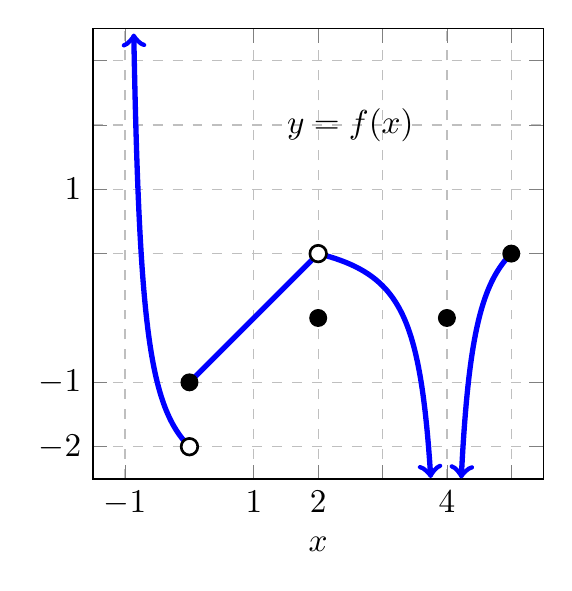
\begin{tikzpicture}[scale=1.2]
  \begin{axis}[
    xlabel={$x$},
    xtick       = {-1,1,2,3,4,5},
    xticklabels = { $-1$, $1$,$2$, ,$4$,},
    ytick       = {-2,-1,1,2,3,4},
    yticklabels = {$-2$,$-1$, ,$1$, , ,},
    samples     = 320,
    domain      = -2.5:5.5,
    restrict y to domain=-2.5:4.5,
    xmin = -1.5, xmax = 5.5,
    ymin = -2.5, ymax = 4.5,
    width = 2.5in, height = 2.5in,
    grid=both, grid style=dashed
  ]
  \node at (2.5,3) {$y=f(x)$};
  % pieces 1 & 2
  \addplot[domain=-1:0, blue, ultra thick, mark=none, <-] {-3+1/(x+1)};
  \draw[blue, ultra thick] (0,-1) -- (2,1);
  \filldraw[white] (0,-2) circle (2.5pt);
  \draw[thick] (0,-2) circle (2.5pt);
  \filldraw (0,-1) circle (2.5pt);
  \filldraw (2,0) circle (2.5pt);
  % piece 3
  %\addplot[domain=2:3, blue, ultra thick, mark=none] {(x-3)^3+2};
  \addplot[domain=2:4, blue, ultra thick, mark=none, ->] {1/(x-4)+1.5};
  \filldraw[white] (2,1) circle (2.5pt);
  \draw[thick] (2,1) circle (2.5pt);
  % piece 4
  \addplot[domain=4:5, blue, ultra thick, mark=none, <-] {-1/(x-4)+2};
  %\addplot[domain=4:5, blue, ultra thick, mark=none] {-7*(x-5)^7+1};
  \filldraw (4,0) circle (2.5pt);
  \filldraw (5,1) circle (2.5pt);
\end{axis}
\end{tikzpicture}

\begin{enumerate}
\item[(a)] $\displaystyle\lim_{x\to0^-} f(x)=$ \\ 
\item[(b)] $\displaystyle\lim_{x\to0^+} f(x)= $
\item[(c)] $\displaystyle\lim_{x\to0} f(x)= $ 
\item[(d)] $\displaystyle\lim_{x\to2^-} f(x)= $ 
\item[(e)] $\displaystyle\lim_{x\to2^+} f(x)= $ 
\item[(f)] $\displaystyle\lim_{x\to2} f(x)=$ 
\end{enumerate}

\begin{enumerate}
\item[(g)] $\displaystyle\lim_{x\to4^-} f(x)=  $  \\
\item[(h)] $\displaystyle\lim_{x\to4^+} f(x)=  $  \\
\item[(i)] $\displaystyle\lim_{x\to4} f(x)=  $  \\
\item[(j)] $\displaystyle\lim_{x\to-1^+} f(x)=  $  \\
\item[(k)] $\displaystyle\lim_{x\to1} f(x)=  $  \\
\end{enumerate}

\newpage 
{\exercise{\target{L1}} The graph of the function $f$ is shown below. Use the graph to estimate the values of the following limits. \\

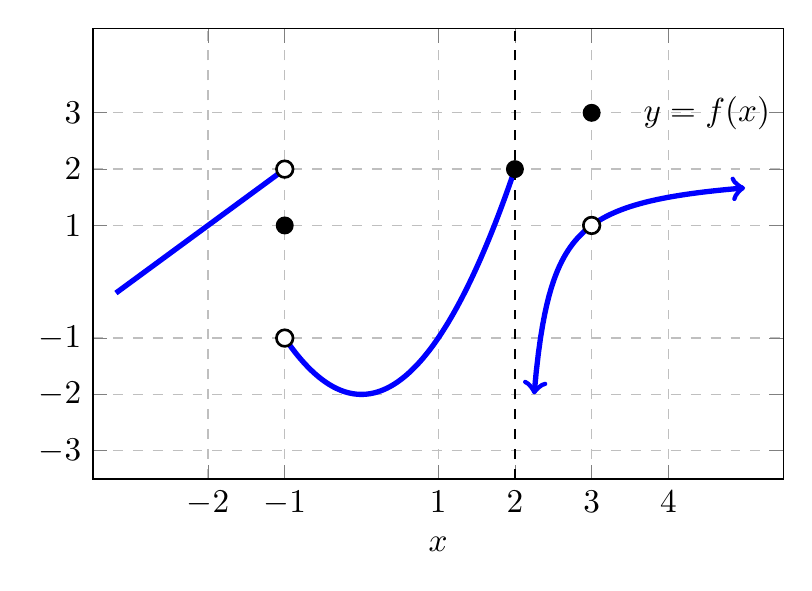
\begin{tikzpicture}[scale=1.2]
  \begin{axis}[
    xlabel={$x$},
    xtick       = {-2,-1,1,2,3,4},
    xticklabels = {$-2$,$-1$,$1$,$2$,$3$,$4$},
    ytick       = {-3,-2,-1,1,2,3},
    yticklabels = {$-3$,$-2$,$-1$,$1$,$2$,$3$},
    samples     = 100,
    domain      = -3.5:5.5,
    restrict y to domain=-3.5:4.5,
    xmin = -3.5, xmax = 5.5,
    ymin = -3.5, ymax = 4.5,
    width = 3.5in, height = 2.5in,
    grid=both, grid style=dashed
  ]
  \node at (4.5,3) {$y=f(x)$};

  % Piece 1: Linear segment (-3 to -1)
  % Ends at (-1, 2)
  \addplot[domain=-3.2:-1, blue, ultra thick, mark=none] {x+3};
  \filldraw[white] (-1,2) circle (2.5pt);
  \draw[thick] (-1,2) circle (2.5pt); % Open circle at (-1, 2)
  \filldraw (-1,1) circle (2.5pt);    % Defined point at (-1, 1)

  % Piece 2: Parabola (-1 to 2)
  % Starts at (-1, -1), Ends at (2, 2)
  \addplot[domain=-1:2, blue, ultra thick, mark=none] {x^2-2};
  \filldraw[white] (-1,-1) circle (2.5pt);
  \draw[thick] (-1,-1) circle (2.5pt); % Open circle at (-1, -1)
  \filldraw (2,2) circle (2.5pt);      % Closed circle at (2, 2)

  % Piece 3: Rational function (2 to 5) with Asymptote at x=2
  % y = -1/(x-2) + 2. Passes through (3, 1). Hole at (3,1).
  \addplot[domain=2.25:5, blue, ultra thick, mark=none, <->] {-1/(x-2) + 2};
  
  % Removable discontinuity at x=3
  \filldraw[white] (3,1) circle (2.5pt);
  \draw[thick] (3,1) circle (2.5pt);   % Hole at (3, 1)
  \filldraw (3,3) circle (2.5pt);      % Defined point at (3, 3)

  % Draw dashed asymptote
  \draw[dashed, thick] (2, -3.5) -- (2, 4.5);

\end{axis}
\end{tikzpicture}

\begin{enumerate}
    \item[(a)] $\displaystyle\lim_{x\to-1^-} f(x)=$
    \item[(b)] $\displaystyle\lim_{x\to-1^+} f(x)=$
    \item[(c)] $\displaystyle\lim_{x\to-1} f(x)=$
    \item[(d)] $\displaystyle\lim_{x\to2^-} f(x)=$
    \item[(e)] $\displaystyle\lim_{x\to2^+} f(x)=$
    \item[(f)] $\displaystyle\lim_{x\to2} f(x)=$
\end{enumerate}

\begin{enumerate}
    \item[(g)] $\displaystyle\lim_{x\to3^-} f(x)=$
    \item[(h)] $\displaystyle\lim_{x\to3^+} f(x)=$
    \item[(i)] $\displaystyle\lim_{x\to3} f(x)=$
    \item[(j)] $\displaystyle\lim_{x\to0} f(x)=$
    \item[(k)] $f(3)=$
\end{enumerate}


\newpage

\section{Exercises C, D and E: Sketching graphs that incorporate limit properties} \setcounter{exercise}{2}
{\exercise{\target{L1}}
\enum{
\item Sketch a graph that satisfies the statements in Group I. and a different graph that satisfies the statements in Group II..\\
\begin{minipage}[t][2in]{0.45\textwidth}
Group I.
    \begin{itemize}
    \item $\displaystyle\lim_{x\to2}f(x) = 1$
    \item $f(2)=3$
    \item $\displaystyle\lim_{x\to4^+} f(x)=\infty$
    \item $\displaystyle\lim_{x\to4^-} f(x)=-\infty$
    \item $f(4)=1$\\
    \end{itemize}
\end{minipage}
%
\hfill
%
\begin{minipage}[t][2in]{0.45\textwidth}
Group II.
    \begin{itemize}
    \item $f$ has a removable discontinuity at $x=1$
    \item $f(1)=3$
    \item $f$ has an infinite discontinuity at $x=3$
    \item $f(3)=1$\\[0.2in]
    \end{itemize}
\end{minipage}
\vfill
\item  What similarities do you notice between the graphs for Group I and Group II Hint: Consider the different kinds of discontinuities in each.
\vfill
}
%
%
\newpage
{\exercise{\target{L1}}
\enum{
\item Sketch a graph that satisfies the statements in Group I. and a different graph that satisfies the statements in Group II..\\
\begin{minipage}[t][2in]{0.45\textwidth}
Group I.
    \begin{itemize}
    \item $\displaystyle\lim_{x\to2+}f(x)=1$
    \item $\displaystyle\lim_{x\to2^-}f(x)=3$
    \item $f(2)=2$
    \item $\displaystyle\lim_{x\to4}f(x)=2$
    \item $f(4)=4$\\
    \end{itemize}
\end{minipage}
%
\hfill
%
\begin{minipage}[t][2in]{0.45\textwidth}
Group II.
    \begin{itemize}
    \item $f$ has a jump discontinuity at $x=1$
    \item $f(1)=3$
    \item $f$ has a removable discontinuity at $x=3$
    \item $f(3)=4$\\[0.2in]
    \end{itemize}
\end{minipage}
\vfill
\item  What similarities do you notice between the graphs for Group I and Group II Hint: Consider the different kinds of discontinuities in each.
\vfill
}
%
%
\newpage
%
\vfill
\newpage
%
{\exercise{\target{L1}}
\enum{
\item Sketch a graph that satisfies the statements in Group I. and a different graph that satisfies the statements in Group II..\\
\begin{minipage}[t][2in]{0.45\textwidth}
Group I.
    \begin{itemize}
    \item $\displaystyle\lim_{x\to2^-}f(x)=2$
    \item $\displaystyle\lim_{x\to2^+}f(x)=3$
    \item $f(2)=2$
    \item $\displaystyle\lim_{x\to4^-}f(x)=\infty$
    \item $f(4)=3$\\
    \end{itemize}
\end{minipage}
%
\hfill
%
\begin{minipage}[t][2in]{0.45\textwidth}
Group II.
    \begin{itemize}
    \item $f(1)=2$
    \item $f$ has a jump discontinuity at $x=1$
    \item $f(3)=3$
    \item $f$ has an infinite discontinuity at $x=3$
    \end{itemize}
\end{minipage}
\vfill
\item  What similarities do you notice between the graphs for Group I and Group II Hint: Consider the different kinds of discontinuities in each.
\vfill
}
%
%

\newpage 

\section{Exercise F: Reflecting about limits and continuity}\setcounter{exercise}{5}
{\exercise{\target{L1}} 
\enum{
\item In terms of limits, what does it mean for $f$ to have a removable discontinuity at $x=a$?

\vfill

\item In terms of limits, what does it mean for $f$ to have a jump discontinuity at $x=a$?

\vfill

\item In terms of limits, what does it mean for $f$ to have an infinite discontinuity at $x=a$?

\vfill

}
\newpage
\section{Exercises G and H: Finding intervals where functions are continuous (or not)}\setcounter{exercise}{6}
{\exercise{\target{L1}}   For the  function $\ds f(x)=\frac{\ln(x+1)}{x-5}$, find one interval where the function is continuous and one interval where the function is {\em not} continuous.  \\\\There at least two ways you can think about answering this question. Pick one of these approaches.\\
\mpageT{.5}{.5}[\hs{.1}]{
\begin{center}{\bf Negative Approach}\end{center}
\enum{
\item We must avoid $\ln(0)$ and $\ln(negative \;\;number)$ When is $x+1\leq0$?
\item We must avoid division by $0$.  When is $x+5=0$?
\item Now use your results from the previous two questions to create an interval where:
\itemI{
\item  The function is continuous (i.e. avoids any of the problem values for $x$ that you just identified) 
\item The function is discontinuous (i.e. contains one of the problem values for $x$ you just identified)
}
}
}{
\begin{center}{\bf Positive Approach}\end{center}
\enum{
\item We are looking for   $\ln(positive \;\;number)$ in order to avoid the problem of the log of zero or a negative number.  When is $x+1>0$?
\item We must avoid division by $0$.  When is $x+5\neq0$?
\item Now use your results from the previous two questions to create an interval where:
\itemI{
\item  The function is continuous (i.e. contains only values of $x$ that satisfy your results from  {\em both}  1) and 2).) 
\item The function is discontinuous (i.e. contains values of $x$ different from your answer to 1) {\em or} different from your answer to 2).)
}
}
}

\newpage
{\exercise{\target{L1}}   For the  function $\ds f(x)=\frac{\sqrt{4-x}}{x+2}$, find one interval where the function is continuous and one interval where the function is {\em not} continuous.  \\\\There at least two ways you can think about answering this question. Pick one of these approaches.\\
\mpageT{.5}{.5}[\hs{.1}]{
\begin{center}{\bf Negative Approach}\end{center}
\enum{
\item We must avoid  $\sqrt{negative \;\;number}$.\\ When is $4-x <0$?
\item We must avoid division by $0$.  When is $x+2=0$?
\item Now use your results from the previous two questions to create an interval where:
\itemI{
\item  The function is continuous (i.e. avoids any of the problem values for $x$ that you just identified) 
\item The function is discontinuous (i.e. contains one of the problem values for $x$ you just identified)
}
}
}{
\begin{center}{\bf Positive Approach}\end{center}
\enum{
\item We are looking for   $\sqrt{positive \;\;number}$ in order to avoid the problem of the square root  of a negative number.  When is $4-x\geq 0$?
\item We must avoid division by $0$.  When is $x+2\neq0$?
\item Now use your results from the previous two questions to create an interval where:
\itemI{
\item  The function is continuous (i.e. contains only values of $x$ that satisfy your results from  {\em both}  1) and 2).) 
\item The function is discontinuous (i.e. contains values of $x$ different from your answer to 1) {\em or} different from your answer to 2).)
}
}
}

\end{document}